\chapter{Introduction}\label{chap:introduction}
% \section{Introduction}
% 2 pages
   \begin{figure}[!ht]
        \centering
        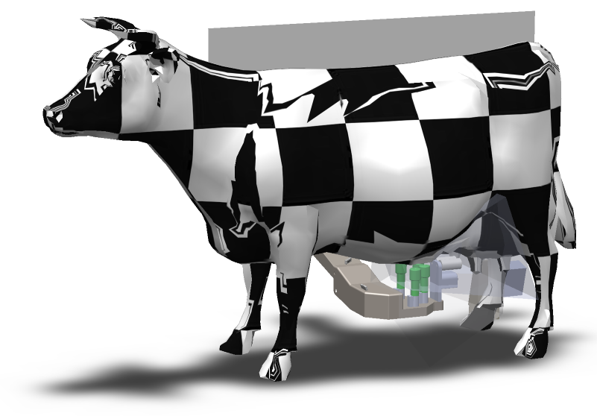
\includegraphics[width=0.7\textwidth]{images/cow_system.png}
        \caption{3D Prototype Model of the Cow Milking Robot}
        \label{fig:cow_fmc}
    \end{figure}
    
\section{Use Case: Improving the Cow Milking Automation}

Aktueller internationaler Stand der Technik
Melkroboter werden schon seit über 20 Jahren erfolgreich in der Landwirtschaft eingesetzt. Die Konzepte der dominierenden Systeme, die am Markt erhältlich sind, wurden in dieser Zeit aber kaum an die neuesten technischen Entwicklungen angepasst. So sind z.B. beim grössten Anbieter Lely die meisten Antriebe auch in der neuesten Version des Melkroboters (Typ Astronaut A5) noch immer elektro-pneumatische Spindelmotoren. Der Grund liegt im günstigeren Preis, sowie in der inhärenten Nachgiebigkeit dieser Antriebe, welche es einfach ermöglicht, einen Schutz der Robotermechanik gegen Kuhtritte zu realisieren. Diese elektro-pneumatischen Antriebe sind aber sehr wartungsintensiv. Insbesondere die Dichtungen dieser Antriebe müssen regelmässig ersetzt werden, so dass das Robotersystem einsatzfähig bleibt. Diese Antriebslösung führt damit auch oft zu ungeplanten Ausfällen des Melkroboters.
In Schweizer Betrieben ist die Herdengrösse in vielen Fällen so, dass mehr als ein Melksystem benötigt wird, die dazu notwendigen zwei Melkroboter aber keinen Platz im bereits vorhandenen Stall haben. Somit ist ein aufwendiger Umbau oder gar ein Neubau des Stalles nötig.

Um mit dem Roboter die Melkbecher an die Zitzen zu bringen muss die Position der Kuh und die exakte Lage der Zitzen erfasst werden. Die aktuellen Melkroboter verwenden dazu meistens 2D Laserscanner. Die Erfassung erfolgt dabei statisch, das heisst, der Roboter bewegt sich während eines Messvorganges nicht. Um mit 2D Scans ein 3D Bild zu erstellen, aus dem die Lage der Zitzen ermittelt werden kann, sind mehrere Messungen notwendig. Das benötigt viel Zeit, und sollte sich die Kuh während der Messung bewegen, muss der Messvorgang sogar wieder neu gestartet werden.

Neuartigkeit der Technik eines modernen Melkroboters

Für den neuen Melkroboter, der im Rahmen dieses Projektes entwickelt werden soll, werden ausschliesslich elektrische Antriebe verwendet. Moderne elektrische Antriebe sind heute viel günstiger als noch vor 20 Jahren, deren Kostennachteil gegenüber elektro-pneumatischen Antrieben ist damit nicht mehr gross. Elektrische Antriebe lassen sich zudem viel präziser regeln. Eine Nachgiebigkeit des Roboters lässt sich mit geeigneten Regelungsstrategien auch mit elektrischen Antrieben realisieren. Der grösste Vorteil von elektrischen Antrieben liegt aber darin, dass sie bei geeigneter Auslegung praktisch wartungsfrei betrieben werden können, was zu einem viel zuverlässigeren System mit höherer Verfügbarkeit führt.
    
Weiter soll für den Roboterarm, welcher die Melkbecher zu den Zitzen führt, eine viel kompaktere kinematische Struktur gewählt werden, beispielsweise ähnlich derjenigen von Scara-Robotern. Ein wesentlicher Vorteil des neuen Gesamtkonzepts ist es, dass im Gegensatz zu den Modellen der Mitbewerber zwei oder mehrere Manipulatoren an einem Basissystem (Pumpe, Kühlung, Lagerung) betrieben werden können. Damit kann das Gesamtsystem kleiner ausgelegt und somit in vielen Fällen in bereits bestehende Stallstrukturen eingebaut werden. Ausserdem kann ein solches System kostengünstiger realisiert werden. Zum Schutz dieses Konzepts hat SLG bereits ein Patent eingereicht (REFERENZ).

Eine weitere Neuartigkeit des neuen Melkroboters findet sich im Bereich der Sensorik, um die Lage der Zitzen zu erfassen. In den letzten Jahren wurden mehrere neue und sehr kostengünstige 3D Kameras auf den Markt gebracht, die für die Erfassung der Lage der Zitzen eingesetzt werden können. Diese Kameras erzeugen direkt 3D Punktewolken mit hoher Auflösung bei Messraten von bis zu 30 Bildern/s. Mit diesen Sensoren kann die Lage der Zitzen dynamisch, das heisst direkt während der Bewegung des Roboters resp. der Melkbecher zu den Zitzen, erfasst werden. Die 3D Messungen müssen dazu in Echtzeit mit der jeweils aktuellen Lage des Roboters verrechnet werden. 

Dies erfordert zwar eine viel aufwändigere Datenverarbeitung auf einer leistungsfähigen Steuerung, dafür kann auf einen 
zeitintensiven, separaten Messvorgang verzichtet werden. Eine dynamische Messung mit modernen Sensoren bietet zudem das Potenzial, wesentlich robuster und zuverlässiger zu sein als die heute eingesetzten Messverfahren.
    
    % \begin{itemize}
    %     \item describe the general need for automated cow milking
    %     \item describe how the problem is currently being solved briefly
    
    %     \item describe the challenges in cow teat recognition: morphology/shapes and movement
    %     \item describe how these methods fail || describe challenges/limitations of current methods (sensors, etc, no memory)
    
    %     \item can solve this problem with computer vision briefly
    
    %     \item describe cow project main driver (The InIT's purpose) (do we mention how expensive current solutions are?)

    % \end{itemize}
\section{Towards 3D Object Detection}
\lipsum[2-5]

    % \begin{itemize}
    %     \item describe advancements in traditional computer vision for image interpretation
    %     \item list shortcomings/challenges we can overcome with computer vision
        
    %     \item describe advancements in computer vision with DL for object detection
    %     \item list shortcomings/challenges we can overcome with computer vision
        
    %     \item shortcoming1: no object permanence | objects out of sight
    %     \item shortcoming2: reliability of only detecting cow teats (?)
    %     \item HELP: shortcoming3: (?) (need to re-read the papers from gio)

    % \end{itemize}
\section{Problem Description}
% \lipsum[2-3]
Die Sutter Landtechnik GmbH (SLG) in Andwil SG und Muolen SG bietet Vertrieb, Installation und Service von technischen Apparaten und Maschinen für die verschiedensten Aufgaben in der Landwirtschaft an. Die Kunden sind Landwirtschaftsbetriebe verschiedenster Grösse in der Deutschschweiz und im nahen Ausland. Nebst den Bereichen Traktoren und Landtechnik (z.B. Erntemaschinen), Hoftechnik (Stalleinrichtungen) gibt es den Bereich Melktechnik, welcher nebst den Melkmaschinen die Kühltechnik und nicht zuletzt auch Melkroboter umfasst. Diverse Maschinen, unter anderem auch Melktechnik, wurden von SLG selber entwickelt und werden auch im eigenen Betrieb hergestellt. Von den rund 50'000 landwirtschaftlichen Betrieben in der Schweiz sind rund 2’000 Kunden von SLG. Dazu kommen noch ca. 200 Betriebe aus dem nahen Ausland dazu. Mit diesen erwirtschaftet SLG mit ihren 25 Mitarbeitern einen Jahresumsatz von ~6.3 MCHF (2018). Alle von SLG installierten und/oder gewarteten Melkroboteranlagen sind vom Typ «Astronaut» von der Niederländischen Firma Lely.

Die Firma Lely mit der Modellreihe Astronaut konnte sich aus den verschiedensten Gründen auf dem Europäischen Markt etablieren und ist mit Abstand Markführer. Der Europäische Markt ist von zwei Marken geprägt wobei die Firma Lely 55% und die Firma DeLaval 30% des Marktes dominieren. In der Schweiz

sind aktuell insgesamt rund 850 Lely Astronaut und rund 300 DeLaval VMS Melkroboter in Betrieb. Der Schweizer Markt wird hierbei klar von der Firma Lely mit ca. 72% Marktanteil dominiert. Die schwache Konkurrenz, sowie der im Verhältnis zu Europa kleine Schweizer Markt führt dazu, dass sich spezifische Anpassungen nur für den Schweizer Markt für die grossen Konzerne nicht lohnen.

In den letzten Jahren hat sich der finanzielle Druck auf die Landwirtschaft in der Schweiz massiv erhöht. Seit 1980 schrumpft die Anzahl der bäuerlichen Betriebe jährlich um rund 1000 Betriebe. Der Schweizer Konsument möchte mehr und mehr biologisch angebaute Produkte und zugleich aber immer günstigere Konsumentenpreise. Die umfangreichen Schweizer Tierschutzbestimmungen, welche europaweit die strengsten sind, verteuern die Tierhaltung zusätzlich. Das alles führt dazu, dass der durchschnittliche Verdienst einer Bauernfamilie jährlich abnimmt. Der Bauernverband fordert daher höhere Unterstützung durch den Staat. Die SLG sieht den Schlüssel für das rentable Führen eines Schweizer Landwirtschaftsbetriebs nicht in höheren staatlichen Zuschüssen, sondern in einem leistungsfähigeren Maschinenpark, welcher spezifisch für den Schweizer Markt, entsprechend der Schweizer Gesetzgebung und für eine biologische und ökoligische Landwirtschaft optimiert ist. Alle heute erhältlichen Robotermelkanlagen sind nicht für biologische Landwirtschaft ausgelegt sondern für die Maximierung des Milchertrages optimiert. Im gesättigten Schweizer Milchmarkt braucht es aber nicht noch mehr Milch, sondern eher fair, biologisch und kosteneffizient hergestellte Milch.

Europaweit ist biologisch produzierte Milch immer noch ein Nischenprodukt. Die SLG ist jedoch überzeugt, dass sich dies in den kommenden Jahren ändern wird, da auch die Konsumenten in Europa immer mehr drauf achten was sie essen und wie Ihr Essen hergestellt wurde. Der Fokus einer Neuentwicklung solle daher nicht auf Maximierung der Milchmenge je Tier liegen, sondern auf Minimierung der Investitionsund Betriebskosten gerichtet sein, und vorallem auch sollten diese neuen Systeme kompromisslos eine biologische Landwirtschaft ermöglichen. Dies beginnt damit, dass den Kühen Zugang zu den Weiden ermöglicht wird.

Die heutigen Robotersysteme sind auf 24/7-Betrieb ausgelegt. Gerade bei kleineren Betrieben ist diese Betriebsart nötig, um die Betriebskosten tief zu halten. Im Gegensatz dazu ist eine wichtige Eigenschaft des neuen Robotersystems, alle Kühe eines Betriebs innerhalb ein bis zwei Stunden melken zu können und somit alle Vorteile eines konventionelles Melkstandes mit den Vorteilen eines Melkroboters zu verbinden. Dazu wird der neue Roboter so dimensioniert, dass mehrere Roboterarme in den Zwischengängen von bestehenden Ställen eingebaut werden können, ohne dass grössere kostenintensive Gebäudeanpassungen nötig werden. Durch den Einbau in den Zwischengängen der Stallung wird es zudem möglich den Einsatz von Kraftfutter zu minimieren, da die Kühe beim Wechsel von den Liegeboxen zu den Fressachsen automatisch den Roboter passieren.

Da die Firma Lely kein Interesse an Produktanpassungen für den Schweizer Mark hatte, hat SLG 2016 die direkten Geschäftsbeziehungen mit Lely beendet und sich für die Entwicklung eines eigenen Robotersystems entschieden. Daher soll in diesem Projekt der Prototyp eines günstigen, modernen Melkroboters passend für die spezifischen Schweizer Anforderungen entwickelt werden, welcher von Sutter Landtechnik GmbH (SLG) selber hergestellt und vermarktet werden kann.

% Als Resultat dieses Forschungsprojekts steht der Prototyp eines modernen Melkroboters, welcher durch seine auf kleinere Betriebe angepasste Konstruktion und aufgrund der eigenen Produktion und dem direkten Vertrieb durch SLG auch in kleineren Landwirtschaftsbetrieben rentabel eingesetzt werden kann. Die Forschungsresultate sind für SLG einfach und zeitnah in ein Produkt umwandelbar, welches direkt im Schweizer Landwirtschaftsumfeld vermarktet werden kann und somit im Bereich Landwirtschaft zu einer besseren, effizienteren und ökologischeren Produktion beitragen wird.

    % \begin{itemize}
        % \item in this work we answer the question: ---
        % \item we start by describing:
        %     \SubItem state of algorithms for cow milking
        %     \SubItem state of algorithms for 3d object detection
        %     \SubItem describe the system is able to localize cow teats in 3d space
        %     \SubItem describe the diverse algorithms we evaluated and tested (?)
        %     \SubItem finally we discuss the outcome of experiments and how to interpret conclusions
        %     \SubItem REWRITE/REUSE THIS SENTENCE FROM THESIS: We do not attempt to solve the specific use case of the ZHAW Summit XL Steel mobile robot, but aim to create an approach which is helpful in a large range of possible scenarios, similar to the way 3D mapping systems already enable robotic interaction today.
    % \end{itemize}
